% !TEX program = xelatex
\documentclass[13pt]{article}
\usepackage{comment}
\usepackage{fontspec}
%\usepackage[utf8]{inputenc}
%\usepackage[vietnamese]{babel}
\usepackage{graphicx}
\usepackage{array}
\usepackage{amsmath, amsfonts}
\usepackage{tikz}
\usepackage{pgfplots}
\usepgfplotslibrary{fillbetween}
\setmainfont{Times New Roman}
\graphicspath{ {./images/} }
\begin{document}
\renewcommand{\figurename}{Hình}
\vfill
\begin{center}
\textbf{ĐẠI HỌC QUỐC GIA TP. HỒ CHÍ MINH}\\
\textbf{TRƯỜNG ĐẠI HỌC BÁCH KHOA}\\
\textbf{KHOA KHOA HỌC ỨNG DỤNG}\\

\includegraphics[scale=0.0625]{logo}\hfil\\
\textbf{\huge\huge BÁO CÁO BÀI TẬP LỚN}\\
\vspace{1cm}
\textbf{MÔN HỌC: GIẢI TÍCH 1}\\
\textbf{GVHD: Lê Thị Yến Nhi}\\
\vspace*{0.5cm}
\textbf{Sinh viên:}\\
\vspace*{0.5cm}
\begin{tabular}{ m{3.75cm}|m{1cm} }
     Họ và tên &  MSSV\cr
    \hline
     Bùi Phan Khánh Duy &    2352170\cr 
     Huỳnh Thiên Phúc &      2352930\cr
     Nguyễn Hoàng Gia Huy &  2352390\cr
     Nguyễn Lê Minh Nhật &   2352860
\end{tabular}
\end{center}
\vspace{\the\dimexpr\paperheight/4\relax}
\section*{LỜI CẢM ƠN}
\par Trước hết, chúng em muốn gửi lời cảm ơn đến cô Lê Thị Yến Nhi, Trường Đại học Bách khoa - ĐHQG-HCM đã tạo điều kiện cho chúng em học hỏi, trang bị đủ kiến thức trong suốt khoá học vừa qua. Sự tận tâm, lời khuyên và nhiệt huyết của họ là nhân tố quan trọng đã truyền cảm hứng cho chúng em, giúp chúng em trình bày bản báo cáo này một cách hoàn thiện và sâu sắc nhất.\\
\par Ngoài ra, chúng em không thể thiếu lời cảm ơn đến những người thân, người bạn đã đóng góp vào bản báo cáo này, dù theo nhiều cách khác nhau. Qua đó, chúng em rất vui lòng được đón nhận sự đóng góp của thầy cô, anh chị và các bạn.
\vfill\newpage
\renewcommand*\contentsname{Mục lục}
\contentsline {section}{\numberline {1}Mở đầu}{4}{}%
\contentsline {section}{\numberline {2}Cơ sở lí thuyết}{5}{}%
\contentsline {subsection}{\numberline {2.1}Mô hình tăng trưởng tự nhiên}{5}{}%
\contentsline {subsection}{\numberline {2.2}Mô hình logistic}{5}{}%
\contentsline {subsection}{\numberline {2.3}Định luật của Newton về sự giảm nhiệt}{6}{}%
\contentsline {subsection}{\numberline {2.4}Thể tích}{7}{}%
\contentsline {subsubsection}{\numberline {2.4.1}Công thức số 1}{7}{}%
\contentsline {subsubsection}{\numberline {2.4.2}Công thức số 2}{7}{}%
\contentsline {subsubsection}{\numberline {2.4.3}Công thức số 3}{7}{}%
\contentsline {subsubsection}{\numberline {2.4.4}Công thức số 4}{7}{}%
\contentsline {subsection}{\numberline {2.5}Độ dài đường cong phẳng - Diện tích mặt tròn xoay}{7}{}%
\contentsline {section}{\numberline {3}Bài toán độ dài cung và diện tích mặt tròn xoay với đường cong tham số}{8}{}%
\contentsline {subsection}{\numberline {3.1}Đạo hàm tại 1 điểm}{8}{}%
\contentsline {section}{\numberline {4}Các ví dụ}{9}{}%
\contentsline {subsection}{\numberline {4.1}Ứng dụng của đạo hàm}{9}{}%
\contentsline {subsubsection}{\numberline {4.1.1}Chi phí cận biên}{9}{}%
\contentsline {subsubsection}{\numberline {4.1.2}Giá trị nhỏ nhất}{9}{}%
\contentsline {subsection}{\numberline {4.2}Ứng dụng của tích phân}{11}{}%
\contentsline {subsection}{\numberline {4.3}Ứng dụng của phương trình vi phân}{12}{}%
\contentsline {section}{\numberline {5}Tài liệu tham khảo}{14}{}%
\newpage
\section{Mở đầu}
Đạo hàm, tích phân và phương trình vi phân là một trong những chuyên đề quan trọng trong chương trình giáo dục bậc THPT và Đại học. Ngoài việc xuất hiện trong sách vở, bài tập, bài kiểm tra thì chúng cũng được ứng dụng trong đời sống hằng ngày rất nhiều. Tiêu biểu có thể kể đến:
\begin{itemize}
    \item Đạo hàm: dùng để tính toán tiếp tuyến của đường cong phẳng, giải thích sự biến thiên tức thời (vận tốc tức thời, cường độ dòng điện tức thời, gia tốc tức thời\dots), chứng minh tính đơn điệu của hàm số, điều kiện để hàm số có cực trị\dots Từ đó có thể ứng dụng vào đời sống như: tốc kế trên xe máy, ứng dụng trong kinh tế sao cho chi phí xây dựng, thiết kế công trình là thấp nhất, tốc độ tăng trưởng kinh tế nhằm đưa ra những quyết định đầu tư đúng đắn\dots
    \item Tích phân: tính diện tích, thể tích của một vật bất kì, tính toán các đại lượng vật lí dựa vào mối liên hệ đạo hàm giữa chúng, tính vi phân\dots
    \item Phương trình vi phân: dùng để miêu tả sự biến thiên của một giá trị theo thời gian, có thể dùng để tính toán liên kết giữa nguyên tử và phân tử, tính toán các chủ đề trong điện tử, tăng trưởng dân số, vật lí (dao động điều hoà), theo dõi sự phát triển của vi sinh vật, vật lí lượng tử, mối liên hệ cung-cầu\dots
\end{itemize}
Trong bài báo cáo này, chúng em trình bày một số ứng dụng trong thực tế của những chuyên đề này nói riêng và giải tích nói chung.
\newpage
\section{Cơ sở lí thuyết}
\subsection{Mô hình tăng trưởng tự nhiên}
\textbf{Bài toán tổng quát:} Kích thước một quần thể $P(t)$ theo thời gian $t$ được mô hình bởi phương trình vi phân $\frac{dP}{dt}=kP(t)$ với điều kiện $P(0)=P_0$ và $k$ là hằng số dương. Giải phương trình tìm $P(t)$.\\
\centerline{\textbf{Giải}}\\
\begin{minipage}{7cm}
Ta có:
\begin{align*}
    &\frac{dP}{dt}=kP\Rightarrow\frac{dP}{P}=kdt\\
    \Rightarrow &\int\frac{dP}{P}=\int kdt\\
    \Leftrightarrow &\ln|P|=kt+C\\
    \Leftrightarrow &|P|=e^C.e^{kt}\\
    \Rightarrow &P=\pm e^C.e^{kt}=C_0e^{kt}\\
    \Rightarrow &P=P_0e^{kt}
\end{align*}
\end{minipage}
\begin{minipage}{7cm}
    \begin{center}
        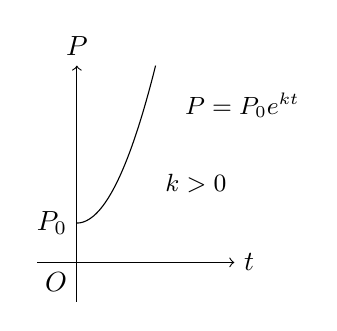
\begin{tikzpicture}
            \node[right] at (1,1) {\small $k>0$};
            \node[right] at (1.25,2) {\small $P=P_0e^{kt}$};
            \node[left] at (0, -0.25) {$O$};
            \node[left] at (0, 0.5) {$P_0$};
            \draw[->] (-0.5, 0) -- (2, 0) node[right] {$t$};
            \draw[->] (0, -0.5) -- (0, 2.5) node[above] {$P$};
            \draw[scale=0.5, domain=0:2, smooth, variable=\x, black]  plot ({\x}, {\x^2+1});
        \end{tikzpicture}
    \end{center}
\end{minipage}
\subsection{Mô hình logistic}
\textbf{Bài toán tổng quát:} Kích thước một quần thể $P(t)$ theo thời gian $t$ được mô hình bởi phương trình vi phân $$\frac{dP}{dt}=kP(t)\bigg(1-\frac{P(t)}{M}\bigg)$$với điều kiện $P(0)=P_0$, $k$ là hằng số dương và $M$ là sức chứa của môi trường. Giải phương trình tìm $P(t)$.\\
\centerline{\textbf{Giải}}\\
Viết lại phương trình: \begin{align*}
    &\frac{M}{P(M-P)}dP=kdt\\
    \Rightarrow &\int\frac{M}{P(M-P)}dP=\int kdt\\
    \Leftrightarrow &\int\bigg(\frac{1}{P}+\frac{1}{M-P}\bigg)dP=\int kdt\\
    \Rightarrow &\ln|P|-\ln|M-P|=kt+C\\
    \Rightarrow &\ln\bigg|\frac{P}{M-P}\bigg|=kt+C\\
    \Rightarrow &\frac{P}{M-P}=C_0.e^{kt}\\
    \Rightarrow &\frac{M-P}{P}=C_1.e^{-kt}\\
    \Rightarrow &\frac{M}{P}-1=C_1.e^{-kt}\\
    \Rightarrow &P=\frac{M}{1+C_1.e^{-kt}}
\end{align*}
\subsection{Định luật của Newton về sự giảm nhiệt}
Theo định luật Newton, tốc độ làm lạnh (giảm nhiệt) của vật thể tỷ lệ với hiệu của nhiệt độ vật thể và nhiệt độ môi trường xung quanh.\\
Gọi $T$ là nhiệt độ của vật, $T_0$ là nhiệt độ của môi trường xung quanh, $k$ là hằng số tỉ lệ ($k<0$). Ta có mô hình phương trình vi phân sau: $$\frac{dT}{dt}=k(T-T_0)$$
\centerline{\textbf{Giải}}\\
Ta có: \begin{align*}
&\frac{dT}{dt}=k(T-T_0)\\
\Rightarrow &\frac{dT}{T-T_0}=kdt\\
\Rightarrow &\int\frac{dT}{T-T_0}=\int kdt\\
\Rightarrow &\ln|T-T_0|=kt+C\\
\Rightarrow &|T-T_0|=e^{kt+C}=e^C.e^{kt}\\
\Rightarrow &T-T_0=\pm e^C.e^{kt}\\
\Rightarrow &T=T_0+C_0.e^{kt}
\end{align*}
\textbf{Cách 2:} Giải theo cách đổi biến\\
Đặt $U=T-T_0\Rightarrow U'=T'\Rightarrow \frac{dU}{dt}=kU$ (giống với mô hình tăng trưởng tự nhiên)\\
$$U=C_0.e^{kt}\Leftrightarrow T-T_0=C_0.e^{kt}\Rightarrow T=T_0+C_0.e^{kt}$$
\subsection{Thể tích}
\subsubsection{Công thức số 1}
Thể tích của vật thể được tạo thành khi quay miền phẳng giới hạn bởi $0\leq y\leq f(x)$, $a\leq x\leq b$ quanh trục Ox là: $$V_x=\int_a^b\pi f(x)^2dx$$
\subsubsection{Công thức số 2}
Thể tích của vật thể được tạo thành khi quay miền phẳng giới hạn bởi $0\leq g(x)\leq y\leq f(x)$, $a\leq x\leq b$ quanh trục Ox là:
$$V_x=\int_a^b\pi (f(x)^2-g(x)^2)dx$$
\subsubsection{Công thức số 3}
Thể tích của vật thể được tạo thành khi quay miền phẳng giới hạn bởi $0\leq y\leq f(x)$, $0\leq a\leq x\leq b$ quanh trục Oy là:
$$V_y=\int_a^b2\pi.x.f(x)dx$$ 
\subsubsection{Công thức số 4}
Thể tích của vật thể được tạo thành khi quay miền phẳng giới hạn bởi $0\leq g(x)\leq y\leq f(x)$, $0\leq a\leq x\leq b$ quanh trục Oy là:
$$V_y=\int_a^b2\pi.x.(f(x)-g(x))dx$$
\subsection{Độ dài đường cong phẳng - Diện tích mặt tròn xoay}
Cho đường cong $C:y=f(x),a\leq x\leq b$, ta có độ dài đường cong $C$ là $$L=\int_a^b\sqrt{1+[f'(x)]^2}dx$$
Khi $C$ quay quanh Ox tạo thành diện tích, ta có $$S_x=2\pi\int_a^b|f(x)|\sqrt{1+[f'(x)]^2}dx$$
\section{Bài toán độ dài cung và diện tích mặt tròn xoay với đường cong tham số}
Cho đường cong $C:x=x(t),y=y(t),t_1\leq t\leq t_2$, ta có:
$$L=\int_{t_1}^{t_2}\sqrt{[x'(t)]^2+[y'(t)]^2}dt$$
$$S_x=2\pi\int_{t_1}^{t_2}|y(t)|\sqrt{[x'(t)]^2+[y'(t)]^2}dt$$
\subsection{Đạo hàm tại 1 điểm}
Cho $y=f(x)$ xác định trong $(a,b)$ với $x_0\in(a,b)$, xét tỷ số
$$\frac{\Delta f(x_0)}{\Delta x}=\frac{f(x)-f(x_0)}{x-x_0}=\frac{f(x_0+\Delta x)-f(x_0)}{\Delta x}$$
Nếu tỷ số trên có giới hạn hữu hạn khi $x\to x_0$ hay $\Delta x\to0$ thì $f$ có đạo hàm tại $x_0$. Đặt
$$f'(x_0)=\lim_{x\to x_0}\frac{\Delta f(x_0)}{\Delta x}$$
\newpage
\section{Các ví dụ}
\subsection{Ứng dụng của đạo hàm}
\subsubsection{Chi phí cận biên}
\par Đặt $C(x)$ là chi phí cần thiết để một công ty sản xuất $x$ sản phẩm, gọi là hàm \textbf{chi phí}. Nếu số sản phẩm tăng từ $x_1$ lên $x_2$, thì chúng ta phải bỏ ra thêm $\Delta C=C(x_2)-C(x_1)$ và độ tăng chi phí là $$\frac{\Delta C}{\Delta x}=\frac{C(x_2)-C(x_1)}{x_2-x_1}=\frac{C(x_1+\Delta x)-C(x_1)}{\Delta x}$$Giới hạn của biểu thức trên khi $\Delta x\to0$, mức độ thay đổi tức thời theo số lượng sản phẩm, gọi là \textbf{chi phí cận biên}.
\par Lấy $\Delta x=1$ và $n$ lớn (để $\Delta x\ll n$), ta có: $$C'(n)\approx C(n+1)-C(n)$$Vậy chi phí cận biên sẽ bằng độ tăng chi phí khi sản xuất thêm 1 sản phẩm.
\par Thường hàm $C(x)$ được coi là một đa thức: $$C(x)=a+bx+cx^2+dx^3$$ với $a$ là chi phí chung (tiền thuê xưởng, bảo dưỡng\dots) và những hạng tử còn lại biểu thị các đại lượng phụ thuộc vào số sản phẩm như chi phí nguyên liệu, nhân công\dots\newline
\par\textbf{Ví dụ:} Chi phí (\$) để sản xuất $x$ sản phẩm là $C(x)=5000+10x+0.05x^2$.\newline
\hspace*{1cm}(a) Tìm mức độ thay đổi của $C$ theo $x$ khi lượng sản phẩm thay đổi\newline
\hspace*{2cm}(i) từ $x=100$ đến $x=105$\newline
\hspace*{2cm}(ii) từ $x=100$ đến $x=101$\newline
\hspace*{1cm}(b) Tìm chi phí cận biên của $C$ tại $x=100$.\newline
\centerline{\textbf{Giải}}\newline
(a) (i) $\frac{C(105)-C(100)}{105-100}=20.25$ (\$/sản phẩm).\newline
\hspace*{0.5cm}(ii) $\frac{C(101)-C(100)}{101-100}=20.05$ (\$/sản phẩm).\newline
(b) $C'(x)=10+0.1x$. Vậy $C'(100)=20$ (\$/sản phẩm).
\subsubsection{Giá trị nhỏ nhất}
\par Trong khoa học máy tính, trí tuệ nhân tạo hoạt động bằng cách ghi nhớ những kiến thức nó đã học được thông qua luyện tập, cứ mỗi một bài tập ta sẽ có hàm $C(x)$ là bình phương độ sai khác giữa đáp án đúng và đáp án mà nó đưa ra. Ta sẽ cố gắng tìm ra giá trị $x$ mà tại đó sai khác là nhỏ nhất.\newline
\par\textbf{Ví dụ:} Giả sử hàm $C(x)=0.2x^4+0.1x^3-x^2+2$. Tìm ra giá trị $x$ sao cho $C(x)$ là nhỏ nhất.\newline
\centerline{\textbf{Giải}}\newline
Ta biết rằng giá trị nhỏ nhất của $C(x)$ sẽ là một trong các cực trị của nó (ta sẽ xét trên toàn bộ tập xác định $\mathbb{R}$), với $C'(x)=0$. Từ đó ta tính được $C'(x)=0.8x^3+0.3x^2-2x$. Cho đạo hàm này bằng 0, giải ra ta được:
\begin{align*}
    &0.8x^3+0.3x^2-2x=0\\
    \Leftrightarrow & x=0\text{ hoặc } 0.8x^2+0.3x-2=0
\end{align*}
Tính được $\Delta=0.3^2-4\times0.8\times-2=6.49>0$, vậy ta có tập nghiệm $S=\{0,-1.78,1.41\}$ (các giá trị đã được làm tròn).\\Ta có:
\begin{align*}
    &f(0)=2\\
    &f(-1.78)\approx0.28\\
    &f(1.41)\approx1.08
\end{align*}
\\
Vậy khi $x\approx-1.78$ thì máy tính đưa ra đáp án sát với thực tế nhất.\\
\begin{figure}
    \caption{Đồ thị $C(x)=0.2x^4+0.1x^3-x^2+2$}
    \begin{center}
        \begin{tikzpicture}[scale=1.0]
            \begin{axis}[ymin=-1,ymax=4,samples=200,axis y line=middle,axis x line=middle,ylabel=$y$,xlabel=$x$]
                \addplot[domain=-4:4, black, thick] {0.2*x^4+0.1*x^3-x^2+2};
            \end{axis}
        \end{tikzpicture}
    \end{center}
\end{figure}
\par\textbf{Ví dụ 3:} Để so sánh độ axit của các dung dịch khác nhau, các nhà hoá học sử dụng pH. Độ pH được xác định theo nồng độ $x$ của các ion hydro trong dung dịch là $$\text{pH}=-\log_{10}x$$
Tìm tốc độ thay đổi của pH ứng với nồng độ ion hydro khi pH là 2.\\
\centerline{\textbf{Giải}}\newline
Ta có $y'=-\frac{1}{x.\ln10}\rightarrow y'(2)\approx-0,217$\\
Vậy tốc độ thay đổi của pH khi $\text{pH}=2$ là $-0,217$.
\subsection{Ứng dụng của tích phân}
\par\textbf{Ví dụ 1}: Một hòn non bộ có dạng như miền giới hạn bởi parabol $y=1-4x^2$, $y=0$, $x\geq0$ quay xung quanh trục Oy. Hòn non bộ được đặt trong hồ nước và nước chiếm 1/4 chiều cao của nó. Đơn vị các trục tính theo mét (m). Tính phần thể tích nổi phía trên mặt nước của hòn non bộ theo $\text{m}^3$.\\
\begin{minipage}{7cm}
\begin{center}
    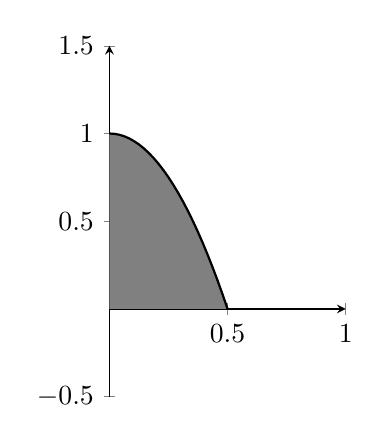
\begin{tikzpicture}[scale=1.0]
        \begin{axis}[width=7cm, ymin=-0.5, ymax=1.5, xmax=1, x=3cm, xtick distance=0.5, axis y line=middle, axis x line=middle]
            \node[right=-11pt] at (50,100) {$y=1-4x^2$};
            \addplot[domain=0:0.5, black, thick, name path=A] {1-4*x^2};
            \addplot[domain=0:0.5, draw=none,name path=B] {0};
            \addplot+[gray] fill between[of=A and B,soft clip={domain=0:0.5}];
        \end{axis}
    \end{tikzpicture}
\end{center}
\end{minipage}
\begin{minipage}{7cm}
    \begin{tikzpicture}[scale=2]
        \def\fcn{1-4*\x*\x};
        \def\phi{10};
        \def\xmin{-0.5}; \def\xmax{0.5};
        \draw[color=black, domain=\xmin:\xmax]
            plot (\x, \fcn) node [above right] {$y = 1-4x^2$};
        \draw[->] (-1,0) -- (1.5,0) node[right]{$x$};
        \draw[->] (0,-0.5) -- (0,1.5) node[right]{$y$};
        \foreach \x in {0, .25, …, \xmax} {
            \tikzset{xyplane/.estyle={cm={1, 0, 0, cos(90 + \phi),(0, \fcn)}}};
            \draw[xyplane, color=black] (0, 0) circle (\x);
        };
    \end{tikzpicture}
\end{minipage}
\centerline{\textbf{Giải}}
Ta có: $y=1-4x^2\Rightarrow x=\pm\frac{\sqrt{1-y}}{2}$.\\
Thể tích nổi phía trên mặt nước là: $$V=\pi\int_\frac14^1\bigg(\frac{\sqrt{1-y}}{2}\bigg)^2dy=\frac9{128}\pi\approx0,22(\text{m}^3)$$
\par\textbf{Ví dụ 2}: Loa phóng thanh có vành nhôm hình dạng như một phần của đường cong $y=\frac2x$, $1\leq x\leq4$, quay xung quanh trục Ox. Nếu đơn vị trên trục toạ độ tính theo decimet (dm), tính diện tích vành loa (theo $\text{dm}^2$).\\
\begin{minipage}{7cm}
    \begin{tikzpicture}[scale=1.0]
        \begin{axis}[width=5cm, ymin=0, ymax=3, xmin=0, xmax=5, x=1cm, xtick distance=1, axis y line=middle, axis x line=middle]
            \draw[dashed] (100,200) -- (100,0);
            \draw[dashed] (400,50) -- (400,0);
            \node[right=-11pt] at (250,125) {$y=\frac2x$};
            \addplot[domain=1:4, black, thick] {2/x};
        \end{axis}
    \end{tikzpicture}
\end{minipage}
\begin{minipage}{7cm}
    
\includegraphics[scale=0.5]{loa}
\end{minipage}\\
\centerline{\textbf{Giải}}
Diện tích vành loa: $$2\pi\int_1^4\bigg|\frac2x\bigg|\sqrt{1+\bigg(-\frac2{x^2}\bigg)^2}dx=22,13(\text{dm}^2)$$
\begin{minipage}{7cm}
\par\textbf{Ví dụ 3}: Bà A thường đi bộ vòng quanh công viên (xem hình) mỗi ngày vào sáng sớm, đơn vị tính trên mỗi trục là \textit{trăm mét}. Bình thường, bà đi một vòng công viên hết khoảng 1 giờ. Hỏi tốc độ trung bình của bà gần với đáp án nào dưới đây nhất?
\end{minipage}
\hspace{0.5cm}
\begin{minipage}{7cm}
    \begin{center}
        \begin{tikzpicture}
            \draw (-1,-1) -- (-1,1); \draw (-1,-1) -- (1,-1); \draw (-1,1) -- (1,1);
            \node[above left] at (-1,0) {$-2$};
            \node[above left] at (0,-1) {$-2$};
            \node[above left] at (0,1) {$2$};
            \node[above left] at (2,0) {$4$};
            \node[above right] at (2,0) {$x=4-0.5y^2$};
            \draw[->] (-2.5, 0) -- (4.5, 0) node[right] {$x$};
            \draw[->] (0, -2.5) -- (0, 2.5) node[above] {$y$};
            \draw[scale=0.5, domain=-2:2, smooth, variable=\y, black]  plot ({4-0.5*\y*\y}, {\y});
        \end{tikzpicture}
    \end{center}
\end{minipage}
\centerline{\textbf{Giải}}
Ta có $f(y)=4-0.5y^2\rightarrow f'(y)=-y$.\\
Độ dài của cung parabol là: $$\int_{-2}^2\sqrt{1+(-y)^2}dx=5,91\text{ (trăm mét)}$$
Tổng quãng đường bà đi là $4\times3+5,91=17,91\approx18$ (trăm mét) $\approx$ 1,8 (km).\\
Tốc độ trung bình là 1,8/1 = 1,8 (km/h).\\\newline
\begin{minipage}{7cm}
    \par\textbf{Ví dụ 4:} Phần thân của một ly rượu vang có dạng một mặt tròn xoay thu được khi quay đường cong $y=\frac{x^2}2$ quanh trục Oy (đơn vị tính của $x$, $y$ là cm). Người ta để một trái anh đào hình cầu đường kính 2cm vào ly như hình vẽ. Sau đó rót rượu vang vào ly từ từ cho đến khi rượu vang \textbf{vừa ngập trái anh đào} thì ngưng (giả sử rằng trái anh đào luôn chạm đáy ly như hình vẽ). Tính thể tích rượu vang có trong ly.
\end{minipage}
\begin{minipage}{7cm}
    \begin{center}
        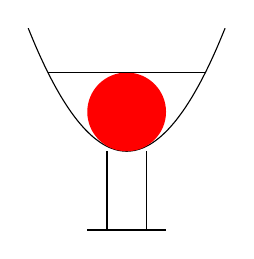
\begin{tikzpicture}
            \draw[scale=0.5, domain=-2.5:2.5, smooth, variable=\x, black]  plot ({\x}, {\x*\x/2});
            \fill[fill=red] (0,0.5) circle(0.5cm);
            \draw (-1,1) -- (1,1);
            \draw (-0.25,0) -- (-0.25,-1); \draw (0.25,0) -- (0.25,-1); \draw (-0.5,-1) -- (0.5,-1);
        \end{tikzpicture}
    \end{center}
\end{minipage}
\centerline{\textbf{Giải}}
Ta có $y=\frac{x^2}{2}\Rightarrow x=\pm\sqrt{2y}$\\
Thể tích rượu và quả anh đào là: $$V_{\text{r+o}}=\pi\int_0^2(\sqrt{2y})^2dy=4\pi(\text{cm}^3)$$
Thể tích quả anh đào là $V_\text{o}=\frac43\pi r^3=\frac{4}{3}\pi\bigg(\frac22\bigg)^3=\frac43\pi(\text{cm}^3)$.\\
Vậy thể tích rượu trong ly là $4\pi-\frac43\pi=\frac83\pi\approx8,4(\text{cm}^3)$.
\subsection{Ứng dụng của phương trình vi phân}
\par\textbf{Ví dụ 1:} Dân số thế giới khoảng 5,707 tỉ người vào năm 1995 và 6,512 tỉ người vào năm 2005. Giả sử tốc dộ tăng trưởng tỉ lệ với quy mô dân số, hay tốc độ tăng trưởng tương đối hầu như không đổi khi quy mô dân số nhỏ. Dựa trên dữ liệu này và sử dụng mô hình đó để dự đoán dân số thế giới năm 2025.\\
\centerline{\textbf{Giải}}
Ta gọi phương trình đại diện dân số thế giới là $$P(t)=P_0.e^{kt}\text{ (tỉ dân)}$$với $t$ là số năm kể từ năm 1995.\\
Năm 2005 ($t=10$), ta có: \begin{align*}
    &P(10)=P_0.e^{k.10}\\
    \rightarrow &6,512=5,707.e^{k.10}\\
    \rightarrow &k=\frac{\ln(6,512/5,707)}{10}\\
\end{align*}
Năm 2025 ($t=30$), ta có: $$P(30)=5,707.e^{k.30}\approx8,479\text{ (tỉ dân).}$$
\par\textbf{Ví dụ 2:} Một CPU khi đang chạy có nhiệt độ $90^\circ$C. Khi máy quá nóng thì quạt tản nhiệt bắt đầu hoạt động, sau 20 phút thì nhiệt độ giảm xuống còn $60^\circ$C trong điều kiện nhiệt độ phòng mở máy lạnh mức $25^\circ$C. Hỏi sau bao lâu thì nhiệt độ giảm còn $40^\circ$C? Biết vận tốc nguội lạnh của CPU trong phòng tỷ lệ với hiệu giữa nhiệt độ của CPU và nhiệt độ phòng.\\
\centerline{\textbf{Giải}}\\
Gọi $y(t)$ là nhiệt độ CPU tại thời điểm $t$ phút, ta có tốc độ  nguội lạnh của CPU tại thời điểm $t$ là $y’(t)$.\\
Theo đề, ta có: \begin{align*}
&y'(t)=k(y(t)-25)\\
\Rightarrow &\frac{dy}{dt}=k(y(t)-25)\\
\Rightarrow &\frac{dy}{y(t)-25}=kdt\\
\Rightarrow &\ln|y(t)-25|=kt+C
\end{align*}
Ta có $y(0)=90$ và $y(20)=60$, suy ra $k\approx-0.03$ và $C\approx4,17$. Ta tìm $t$ khi $y(t)=40$: $$\ln|40-25|=kt+C\Rightarrow t\approx47,4(\text{phút})$$
\par\textbf{Ví dụ 3:} Một loại virus máy tính có tốc độ tự phát tán tại thời điểm $t$ tỷ lệ thuận với số virus hiện tại ở thời điểm đó. Giả sử số lượng virus ban đầu là 2 con, sau 10 giờ là 50 000 con. Xác định số lượng virus sau 1 ngày.\\
\centerline{\textbf{Giải}}\\
Số lượng virus sau $t$ giờ là $P=P_0.e^{kt}$. Theo đề, ta có:
\begin{itemize}
    \item $P_0=2$
    \item $t=10$ thì $P=50 000\Rightarrow k\approx1,01$
\end{itemize}
Vậy sau 1 ngày số lượng virus là khoảng 71 793 647 187 con.\\
\par\textbf{Ví dụ 4:} Một A.I sử dụng hệ thống mạng nơron để học dựa trên dữ liệu hình ảnh gồm 20 000 tấm. Thời điểm ban đầu, A.I học được 20 tấm ảnh. Sau 30 giây A.I học được 500 tấm ảnh. Nhờ hệ thống mạng nơron, A.I càng học thì tốc độ học càng tăng, tỷ lệ với số lượng hình ảnh đã học. Hỏi sau bao lâu A.I học hết 20 000 tấm ảnh?
\centerline{\textbf{Giải}}\\
Gọi $a(t)$ là số lượng hình ảnh A.I đã học được sau $t$ giây, vậy ta có $a'(t)$ là tốc độ A.I học từ các hình ảnh tại thời điểm $t$.\\Theo đề, ta có: \begin{align*}
&a'(t)=ka(t)\\
\Rightarrow &\frac{da}{dt}=kdt\\
\Rightarrow &\ln(a)=kt+C\\
\end{align*}
Với $a(0)=20$, $a(30)=500$, vậy ta có $k\approx1,07$ và $C\approx2,996$.\\Giải $t$: $$a(t)=20000\Rightarrow t\approx64,38(\text{giây})$$
Vậy sau khoảng 64,38 giây thì A.I học được 20 000 tấm ảnh.
\section{Tài liệu tham khảo}
\begin{itemize}
    \item \textit{Calculus} - J. Stewart (6th edition)
\end{itemize}
\end{document}